\chapter{Evaluierung des Conversational Agent Prototyps} \label{Kapitel5}
\chaptermark{Evaluierung}
Zur Beantwortung von RQ1 und RQ2 wurde eine Umfrage durchgeführt. 
Der Teilnehmer wurde gebeten einen Online-Fragebogen auszufüllen sowie 
die Interaktion des Dialogs und die Interaktion des Quiz-Spiels mit Vicky 
in einem Chatgespräch durchzuführen. 
Im Folgenden wird zunächst der Aufbau des Fragebogens beschrieben sowie die darin 
enthaltende Itemauswahl anhand von Literatur begründet (Kapitel 5.1). 
Anschließend folgen in Kapitel 5.2 die Art und Weise der Datenerhebung und das Ergebnis der Studie. 

\section{Studiendesign zum Prototypen} \label{Kapitel5.1}

Ziel der Studie ist die Erforschung, ob durch eine dialogbasierte Interaktion 
zwischen dem Teilnehmer und dem CA Vicky
der Lernstil des Teilnehmers identifiziert werden kann. 
Des Weiteren wird geprüft, inwiefern das Motivationsverhalten 
des Teilnehmers durch die Interaktion mit Vicky beeinflusst werden kann.
Dies ist relevant, um RQ1 und RQ2 zu beantworten.
Darüber hinaus wird zusätzlich die Möglichkeit der Identifikation des Lernstils anhand 
eines Quiz-Spiels zwischen Teilnehmer und Vicky untersucht.
Des Weiteren wird die persönliche Einstellung und Wahrnehmung des Teilnehmers gegenüber Vicky 
analysiert. Die Tabelle \ref{tab:/AufbauFragebogen} zeigt den allgemeinen Aufbau des Fragebogens \footnote{Die Umfrage-Struktur ist als Iss-Format auf dem beigelegten USB-Stick vorzufinden.}.

\begingroup
\footnotesize 
\begin{longtable}{|m{3cm}|m{12cm}|}
    \hline
    \rowcolor[HTML]{EFEFEF} 
    \centering \textbf{Index} & \centering \arraybackslash \textbf{Teilbereich}\\    \hline \hline
    \centering 0 & Willkommensseite                     \\ \hline
    \centering 1 & Soziodemographische Fragen zur Person                    \\ \hline
    \centering 2 & Hinweise zur Interaktion \& Fragen zur Verständlichkeit mit Vicky \\ \hline
    \centering 3 & Fragen zur persönlichen Einstellung und Wahrnehmung zu Vicky \& Lernstilklassifikation                \\ \hline
    \centering \arraybackslash 4 & Messung der Lernmotivation                       \\ \hline
    \caption[Allgemeiner Aufbau des Fragebogens]{Allgemeiner Aufbau des Fragebogens (eigene Darstellung)} 
    \label{tab:/AufbauFragebogen}
\end{longtable}
\endgroup

Auf der Willkommensseite folgt eine kurze Einführung in das Thema sowie einer Definitionserklärung 
des Conversational Agents. Neben allgemeinen Informationen zur Umfrage (Dauer, Anonymisierung der Daten, 
Datenschutzerklärung) werden die Rahmenbedingungen des Experiments erklärt. 
Es wird darauf hingewiesen, dass zwei Interaktionen (Dialog und Quiz-Spiel) 
mit dem CA Vicky folgen und bei jeder erfolgreichen Interaktion der Lernstil ermittel wird. 

\textbf{Teilbereich 1:}

Der Fragebogen startet mit Fragen zur Person, diese beziehen sich dabei auf 
das Alter, auf das Geschlecht, bei Studenten auf das Studienfach und auf den höchsten erreichten Bildungsabschluss.
Um Rückschlüsse auf Sprachbarrieren während der Interaktion mit Vicky nachvollziehen zu können,
wurde zusätzlich das Englischsprachniveau abgefragt.

\textbf{Teilbereich 2:}

Dieser Abschnitt der Umfrage bezieht sich auf die Interaktion mit Vicky. 
Es wurden allgemeine Hinweise zum Vorgehen mit Vicky beschrieben. Darunter fielen: 
Start der Konversation,
Fragen, die der Proband während der Interaktion mit Vicky immer stellen kann,
die Nutzung des Refresh-Buttons, dass Vicky Verneinungen 
von Antworten untersagt, dass einige Antworten auf die Quiz-Fragen ein bestimmtes Format
verlangen sowie die Beantwortung der Fragen entweder durch das Textfeld oder via Button erfolgen kann. 
Anschließend folgt eine Verlinkung zur Interaktion mit Vicky. 
Sobald der Teilnehmer auf den Link klickt, öffnet sich in einem separaten Tab ein
Chatfenster. Der Teilnehmer kann nun die Interaktion mit Vicky durch ein \glqq Hello\grqq{}
beginnen. Nach der Interaktion mit Vicky folgen im zweiten Teilbereich des Fragebogens weitere Fragen 
bezüglich der Verständlichkeit des Gesprächs mit Vicky. Es wurde gefragt: 
\begin{itemize}
    \item \glqq War während des Dialogs eine Frage von Vicky für Sie unverständlich? Wenn Ja, welche?\grqq{}
    \item \glqq Hätten Sie während des Dialogs gerne eine Rückfrage gestellt? Wenn ja, welche?\grqq{}
    \item \glqq Wie fanden Sie den Schwierigkeitsgrad der Fragen des Quiz-Spiels?\grqq{}
    \item \glqq Welche Quiz-Fragen des Spiels fanden Sie unverständlich und wann hätten Sie sich eine bessere Hilfsoption gewünscht? Begründen Sie.\grqq{} (Mehrfachauswahl möglich)
    \item \glqq Haben Sie lieber über Buttons oder über das freie Textfeld geantwortet? Begründen Sie bitte kurz.\grqq{}
    \item \glqq Bestand während der Konversation mit Vicky der Drang abzubrechen?\grqq{} 
\end{itemize}
Diese Fragen wurden gestellt, um zu überprüfen, inwiefern das Erlebnis mit 
Vicky für die Probanden positiv oder negativ war. 

\textbf{Teilbereich 3:} 

Dieser Abschnitt stellt den Hauptteil der Umfrage dar. 
Zuerst wird nach der subjektiven Erfahrung des Teilnehmers, die er allgemein
mit Chatbots bislang gemacht hat, gefragt. Dazu sollte er sein Empfinden zu den folgenden Aussagen 
auf einer Likert-Skala von 1 (Stimme der Aussage gar nicht zu) - 7 (Stimme der Aussage voll zu) \footnote{Die Einstellung bezüglich der Likert-Skala bleibt über die ganze Umfrage hinweg gleich.}
einstufen:
\begin{itemize}
    \item \glqq Ich würde sagen, dass ich erfahren im Umgang mit Chatbots bin.\grqq{} 
    \item \glqq Ich benutze Chatbots regelmäßig.\grqq{} 
    \item \glqq Andere würden sagen, dass ich Erfahrung mit Chatbots habe.\grqq{} 
\end{itemize}
Diese subjektive Einschätzung dient zur Validierung, inwiefern positive bzw. negative Beurteilungen 
bezüglich Vicky auf Unkenntnisse im Umgang mit Chatbots zurückgeführt werden können. 

Um eine gernerelle persönliche Einstellung und Wahrnehmung des Teilnehmers gegenüber Vicky zu messen, 
wurde auf die Erfahrung des Teilnehmers, die er mit Vicky erlebt hat, eingegangen.
Somit wird der Proband erneut gebeten 
seine Einschätzung auf einer Likert-Skala anzugeben, inwiefern die weiteren Aussagen auf ihn passen. 
Die Items sind mit Literaturnachweis im Anhang \ref{Umfrage} zu finden.

Anschließend wurde der Teilnehmer nach seinem identifizierten Lernstil sowie 
nach seiner Meinung, ob er sowohl nach der ersten Interaktion (Dialog) als auch nach 
der zweiten Interaktion (Quiz-Spiel) richtig eingeschätzt wurde, gefragt. Falls nicht, 
konnte er seine persönliche Einschätzung bezüglich des Lernstils in einem 
Kommentarfeld mitteilen. Diese Fragen sind relevant, um RQ1 der vorliegenden 
Arbeit zu beantworten. 

Zum Schluss wurde der Teilnehmer gebeten drei positive und negative Aspekte über die 
Interaktion mit Vicky zu nennen. Des Weiteren wurde nach weiteren Wünschen, Ideen oder Anregungen über
die Weiterentwicklung von Vicky gefragt. 

\pagebreak

\textbf{Teilbereich 4:}

Dieser letzte Abschnitt der Umfrage dient zur Messung der Lernmotivation im 
Umgang mit einem CA und schließlich als Unterstützung zur Beantwortung von RQ2.
Die Items dienen der Messung der Lernmotivation, welche
sich auf die Dimensionen des ARCS-Modell von Keller(1984) sowie auf den situativen Faktor des Rahmenmodells von Rheinberg u.a. (2000) (vgl. Kapitel \ref{Lernmotivation})
beziehen. Der Proband wurde erneut gebeten anzugeben, inwieweit er den unten aufgeführten Aussagen auf einer Likert-Skala zustimmt. 
Die Items wurden eigenständig erstellt. Sie sind im Anhang \ref{ARCSITEMS} \& \ref{SF} zu finden.

Der Fragebogen endet mit den beiden offenen Fragen:
\begin{itemize}
    \item \glqq Stellen Sie sich vor, Sie würden einen CA nutzen,
    der Sie persönlich beim Lernen begleitet, und noch weitere Funktionalitäten
    haben könnte als den Lernstil zu klassifizieren.
    Bitte beschreiben Sie, inwiefern Sie das Gespräch mit Vicky als motivierend oder
    unmotivierend wahrgenommen haben. Begründen Sie gerne Ihre Wahrnehmung dazu.\grqq{} 
    \item \glqq Nach ihrer Erfahrung mit Vicky: Wie würden Sie die Anwesenheit 
    eines virtuellen Begleiters beim Lernen empfinden, der noch weitere Funktionalitäten haben 
    könnte als den Lernstil zu klassifizieren?\grqq{}.
\end{itemize} 

Diese Fragen wurden gestellt, um zum einen Gründe für eine motivierende/ unmotivierende Wirkung der 
Interaktion mit Vicky zu erfahren und zum anderen 
Erkenntnisse über eine Einführung eines virtuellen Begleiters 
in das Lernverhalten zu gewinnen.

\section{Auswertung der Umfrage} \label{Kapitel5.2}

Für die Datenerhebung wurde die Web-Anwendung \glqq LimeSurvey\grqq{} genutzt.
Zuerst wurde ein Pre-Test mit fünf Personen gemacht, um die Umfrage sowie die Interaktion mit 
Vicky auf Verständlichkeit, Korrektheit und technischer Machbarkeit zu prüfen.
Es wurden Rechtschreibfehler korrigiert und unverständliche Sätze umformuliert.
Außerdem wurde eine Quiz-Frage aus dem Quiz-Spiel aufgrund von mathematischer Ungenauigkeit 
entfernt. Des Weiteren konnte mithilfe der Testpersonen die Dauer der Interaktion und der Umfrage eingeschätzt werden.

Für die Umfrage wurde ein betreutes Experiment vorgesehen. Es wurde eine Teilnehmerliste
mit verschiedenen Terminen, in der sich 
Studierende der TU-Braunschweig eintragen konnten, angeboten. Diese wurde über verschiedene Wege verbreitet. 
Die Teilnehmerliste wurde u.a. über den Mail-Verteiler der TU Braunschweig, über das StudIP-Forum, über Vorlesungsveranstaltungen und 
soziale Netzwerke verteilt. Darüber hinaus wurden vereinzelte Termine über soziale 
Messengers verabredet. Bei dem Experiment erhielten die Teilnehmer den Link zur Umfrage. 
Während der Bearbeitungszeit der Umfrage konnten sie Rückfragen zu technischen Problemen
und allgemeinen Unklarheiten stellen. Nachdem ein Teilnehmer die Interaktionen durchgeführt hat, wurden die 
Trainingsdaten angepasst, sodass ein robusterer Prototyp mit der Zeit entstand. \\
Die Datenerhebung fand im Zeitraum vom 19.12.2021 bis zum 10.01.2022 statt. Insgesamt haben 25 Personen an der Umfrage teilgenommen und diese
vollständig abgeschlossen. Dieser Stichprobenumfang ist sehr klein. Für repräsentative Ergebnisse, 
welche auf die Grundgesamtheit übertragen werden können, gilt als Faustregel n $\geq$ 30.
Für detaillierte Ergebnisse, welche auf die Grundgesamtheit übertragen werden sollen, sollte der 
Stichprobenumfang zudem wesentlich größer als 30 sein. \parencite[71]{schöneck.2015} 
In der Umfrage wurden Likert-Skalen von eins bis sieben verwendet. 
Die Zahlen kennzeichnen, inwiefern der Befragte der Aussage zustimmt
(1 = Stimme der Aussage gar nicht zu; ...; 7 = Stimme der Aussage voll zu).

Die Auswertung wurde mit dem Tool \glqq Excel\grqq{} sowie \glqq SPSS-Statistics\grqq{} durchgeführt. \footnote{Beide Dateien sind auf dem USB-Stick zu finden.}
Für eine verständlichere visuelle Darstellung und Interpretation der Likert-Skalen wurden die
statistischen Kennzahlen \textbf{Mittelwert (MW)} und \textbf{Standardabweichung (SD)} genutzt,
um Tendenzen zu bestimmen. Für die Auswertung der offenen Fragen wurde eine 
induktive Kategoriedefinition verwendet. Sie ist von der deduktiven Kategoriedefinition 
abzugrenzen und unterscheidet sich dadurch, dass die Kategorisierung direkt aus dem
dokumentierten Material und nicht auf Basis einer theoretischen Überlegung erfolgt. Mithilfe
der induktiven Kategoriebildung können 
die tatsächlichen Äußerungen der Probanden ohne Vorannahmen des Forschers analysiert werden. \parencite[85 f.]{Mayring.2015}
Für die Bildung der Kategorien wurde sich an dem Vorgehen von Kuckartz (2018) orientiert. 
Dabei wurden die Textpassagen beim ersten Lesen mindestens einer Kategorie zugeordnet. Bei einem weiteren Lesevorgang 
wurden die bereits zugeordneten Kategorien überprüft und ggf. nachgebessert. \parencite[102 ff.]{Kuckartz.2018}
Am Ende dieses Kapitels ist eine Korrelationsanalyse aufgeführt, auf welche sich im Folgenden immer 
wieder bezogen wird, um Annahmen über bestimmte Wirkungsweisen treffen zu können.

Im Folgenden wird zuerst eine Reliabilitätsanalyse durchgeführt. Anschließend werden die einzelnen Teilbereiche der Umfrage deskriptiv ausgewertet.

\textbf{Reliabilitätsanalyse}

Zunächst wurde eine Reliabilitätsanalyse über die verwendeten Items zur Einschätzung der Wahrnehmung von Vicky sowie
der Items zur Messung der Lernmotivation durchgeführt.
Cronbachs Alpha wurde berechnet, um die Items auf interne Konsistenz zu testen. 
Des Weiteren wurde auch die korrigierten Item-Skala-Korrelationen und die Veränderung von Cronbachs Alpha durch eine mögliche Item-Elimination 
ermittelt. Cronbachs Alpha wird auch als Homogenitätsindex bezeichnet. \parencite[291]{Eckstein.2004}
Die nachfolgenden Tabellen repräsentieren die Ergebnisse. \\

\begingroup
\footnotesize 
\begin{longtable}{|m{8cm}|m{2cm}|m{2cm}|m{2cm}|}
    \hline
    \rowcolor[HTML]{EFEFEF} 
    \centering \textbf{Item} &   \centering \textbf{Cronbachs Alpha}  &\centering \textbf{Item-Skala-Korrelation} &\centering \arraybackslash \textbf{Cronnachs Alpha, wenn weggelassen}\\    \hline \hline
     Ich habe Vicky menschenähnlich wahrgenommen.& 0.985 & 0.962 & 0.983                    \\ \hline 

    Ich habe Vicky lebensecht wahrgenommen. & 0.985 & 0.963 & 0.984                    \\ \hline

     Ich habe Vicky natürlich wahrgenommen.& 0.985 & 0.963 & 0.984                     \\ \hline

     Ich fand Vickys Antworten elegant. & 0.985& 0.775 & 0.986                    \\ \hline

     Ich habe ein Gefühl des menschlichen Kontakts gespürt.& 0.985 & 0.966 & 0.983                     \\ \hline

     Ich habe ein Gefühl der menschlichen Wärme gespürt.& 0.985& 0.963 & 0.984                    \\ \hline

     Ich habe ein Gefühl der persönlichen Beziehung gespürt.& 0.985& 0.969 & 0.983                   \\ \hline

      Ich habe ein Gefühl der Kontaktfreudigkeit gespürt. & 0.985& 0.953 & 0.984                  \\ \hline

     Ich denke, Vicky interagiert wie eine Person.& 0.960 & 0.985& 0.984                    \\ \hline

     Ich kann Vicky vertrauen.& 0.985 & 0.916 & 0.984                   \\ \hline

     Ich denke, Vicky ist verlässlich. & 0.985& 0.937 & 0.984                   \\ \hline

     Vicky ist transparent.& 0.985& 0.714 & 0.986                     \\ \hline

     Ich habe Vicky als unmenschlich wahrgenommen.& 0.985& 0.965 & 0.984                    \\ \hline

     Ich habe Vicky als seltsam wahrgenommen. & 0.985& 0.954 & 0.984                    \\ \hline

     Ich habe Vicky als unsympathisch wahrgenommen. & 0.985& 0.821 & 0.985                    \\ \hline

     Ich habe Vicky als unangenehm wahrgenommen. & 0.985& 0.835 &  0.985                \\ \hline

    \caption[Reliabilitätsanalyse der Items zur Wahrnehmung von Vicky]{Reliabilitätsanalyse der Items zur Wahrnehmung von Vicky (eigene Darstellung)} 
    \label{tab:/Reliabilitätsanalyse_Wahrnehmung}
\end{longtable}
\endgroup

\pagebreak
\begingroup
\footnotesize 
\begin{longtable}{|m{8cm}|m{2cm}|m{2cm}|m{2cm}|}
    \hline
    \rowcolor[HTML]{EFEFEF} 
    \centering \textbf{Dimension: Item} &   \centering \textbf{Cronbachs Alpha}  &\centering \textbf{Item-Skala-Korrelation} &\centering \arraybackslash \textbf{Cronnachs Alpha, wenn weggelassen}\\    \hline \hline
     \textbf{A:} Vicky zu antworten hat mir Spaß gemacht. & 0.970 & 0.957 & 0.950                    \\ \hline 

      \textbf{A:} Die Interaktion mit Vicky fiel mir leicht.  & 0.970 & 0.924 & 0.965                    \\ \hline

     \textbf{A:} Ich könnte noch länger mit Vicky kommunizieren. & 0.970  & 0.951 & 0.954                     \\ \hline\hline


     \textbf{R:} Ein CA könnte mir helfen öfter zu lernen. & 0.996 & 0.986 & 1                    \\ \hline 

      \textbf{R:}  Ein CA könnte mir helfen frühzeitiger mit dem Lernen zu beginnen.  & 0.996 & 0.997 & 0.992                    \\ \hline

     \textbf{R:} Ein CA könnte mir beim Erkennen meiner eigenen Stärken und Schwächen helfen. & 0.996  & 0.997 & 0.992                     \\ \hline\hline


     \textbf{C:} Ein CA könnte mir bei meinem Lernerfolg helfen, welcher größtenteils auf meinen eigenen Bemühungen basiert. & 0.992 & 0.988 & 0.987                    \\ \hline 

      \textbf{C:}  Ein CA könnte mir beim Setzen von Lernzielen helfen, welche ich durch meine eigenen Bemühungen erreiche.  & 0.992 & 0.982 & 0.991                    \\ \hline

     \textbf{C:} Ein CA könnte mir bei der Strukturierung meines Lernens helfen. & 0.992  & 0.985 & 0.988                     \\ \hline\hline


     \textbf{S:} Die Interaktion mit Vicky hat mich während des Quiz-Spiels motiviert. & 0.898 & 0.831 & 0.830                    \\ \hline 

      \textbf{S:}  Ein CA könnte mir bei der Aufrechterhaltung der Motivation helfen.  & 0.898 & 0.689 & 0.965                    \\ \hline

     \textbf{S:} Ein CA könnte mir helfen im richtigen Tempo zu lernen. & 0.898  & 0.903 & 0.770                     \\ \hline\hline

    \caption[Reliabilitätsanalyse der Items des ARCS-Modells]{Reliabilitätsanalyse der Items des ARCS-Modells (eigene Darstellung)} 
    \label{tab:/Reliabilitätsanalyse_ARCS}
\end{longtable}
\endgroup

Beide Tabellen weisen einen Homogenitätsindex von über 0.89 auf, was 
als exzellent zu bewerten ist. \parencite[344]{blanz.2021} 
Die Spalte der korrigierten Item-Skala-Korrelation, welche angibt, inwiefern die Items untereinander 
korrelieren, zeigt für alle Items einen Wert von größer als 0.68 auf und können somit als gute Werte 
interpretiert werden, da gute Werte eine Korrelation von 0.30 oder mehr aufweisen. \parencite[344]{blanz.2021} 
Cronbachs Alpha kann durch das Weglassen von einzelnen Items verbessert werden. Da in allen 
Fällen der Homogenitätsindex schon sehr hoch ist, wurde darauf verzichtet.
Insgesamt weist der Fragebogen damit ein valides Konstrukt auf.

\pagebreak

\textbf{Deskriptive Auswertung der Fragen zur Person (Teilbereich 1): }

Die folgende Tabelle \ref{tab:/Auswertung_Angaben_zur_Person} zeigt 
die soziodemographische Verteilung der Stichprobe (n = 25) für ein besseres 
Verständnis der Studienergebnisse.

\begingroup
\footnotesize 
\begin{longtable}{|m{4cm}|m{10cm}|}
    \hline
    \rowcolor[HTML]{EFEFEF} 
    \centering \textbf{Item} & \centering \arraybackslash \textbf{Auswertung}\\    \hline \hline
    \centering Alter & MW = 26,72                     \\ \hline
    \centering Geschlecht & Männlich: 17 (68 \%), Weiblich: 8 (32 \%)                 \\ \hline
    \centering Studiengang & Wirtschaftsinformatik: 8 (32 \%), Informatik: 1 (4 \%), Betriebswirtschaftslehre: 4 (16 \%), Technologie-orientiertes-Management: 1 (4 \%), Wirtschaftsingenieurwesen: 1 (4 \%), Lehramt: 2 (8 \%), 
    Maschinenbau: 1 (4 \%), Medizin: 1 (4 \%), Jura: 1 (4 \%), Physiotherapie: 1 (4 \%), Kommunikation: 1 (4 \%), Sozialwissenschaften: 1 (4 \%), Nachhaltigkeitsrecht: 1 (4 \%), Keinen: 1 (4 \%)       \\ \hline
    \centering Höchster Bildungsabschluss & Abitur: 10 (40 \%), Ausbildung: 1 (4 \%), Bachelor: 11 (44 \%), Master/Diplom: 3 (12\%)               \\ \hline
    \centering \arraybackslash Englischsprachniveau & A2: 1 (4 \%), B1: 4 (16 \%), B2: 16 (64 \%), C1: 3 (12 \%), C2: 1 (4 \%)             \\ \hline
    \caption[Auswertung: Angaben zur Person]{Auswertung Angaben zur Person (eigene Darstellung)} 
    \label{tab:/Auswertung_Angaben_zur_Person}
\end{longtable}
\endgroup

RQ1 zielt auf allgemein Lernende ab, sodass für die Beantwortung dieser Fragestellung unterschiedliche 
Studiengänge in Betracht gezogen werden sollten.
Trotz des Großteils an Lernenden der Wirtschaftsinformatik (32 \%), zeigt die 
Auswertung eine Vielfalt an Studiengängen auf.
Der Dialog zwischen dem Teilnehmer und Vicky ist auf Englisch, deshalb wurde der Teilnehmer nach einer Einschätzung seines Englischsprachniveaus befragt.
Die überwiegende Anzahl an Teilnehmern verfügt über Englischkenntnisse, die für den akademischen
Bereich geeignet sind. \footnote{\url{https://www.spotlight-online.de/englisch-lernen-ratgeber/welches-englisch-sprachniveau-habe-ich}, aufgerufen am 11.01.2022}

\textbf{Deskriptive Auswertung der Fragen zur Interaktion mit Vicky (Teilbereich 2): }

Die nächste Tabelle \ref{tab:/Interaktion_mit_Vicky} bezieht sich auf die Auswertungsergebnisse der Interaktion zwischen Teilnehmer und Vicky.
\begingroup
\footnotesize 
\begin{longtable}{|m{4cm}|m{10cm}|}
    \hline
    \rowcolor[HTML]{EFEFEF} 
    \centering \textbf{Item} & \centering \arraybackslash \textbf{Auswertung}\\    \hline \hline
    \centering War während des Dialogs eine Frage von Vicky für Sie unverständlich?  &  Nein: 25 (100 \%)         \\ \hline
    \centering Hätten Sie während des Dialogs gerne eine Rückfrage gestellt? & Nein: 24 (96 \%), Ja: 1 (4 \%) Wie sicher bist du dir bei meinem Lernstil? (vgl. Anhang \ref{tab:/Kommentare_Teilbereich_2}: 1)          \\ \hline
    \centering Schwierigkeitsgrad der Fragen des Quiz-Spiels? 1: zu leicht 7: zu schwer & MW = 5,08 (SD = 1,18)          \\ \hline
    \centering Welche Quiz-Fragen des Spiels fanden Sie unverständlich und deshalb hätten Sie sich eine bessere Hilfsoption gewünscht? & Q2: 1 (4 \%), Q3: 1 (4 \%), Q4: 4 (16 \%), Q5: 1 (4 \%), Q6: 2 (8 \%), Q7: 3 (12 \%), Q8: 1 (4 \%), Keine: 18 (72 \%)  \\ \hline    
    \centering  Haben Sie lieber über Buttons oder über das freie Textfeld geantwortet? & Buttons: 9 (36 \%), Textfeld: 3 (12 \%), Beides: 13 (52 \%)         \\ \hline    
    \centering \arraybackslash Bestand während der Konversation mit Vicky der Drang abzubrechen?  & Ja: 4 (16 \%), Nein: 21 (84 \%)          \\ \hline
    \caption[Auswertung: Interaktion mit Vicky]{Auswertung: Interaktion mit Vicky (eigene Darstellung)} 
    \label{tab:/Interaktion_mit_Vicky}
\end{longtable}
\endgroup

Während des Gesprächs wurden die Fragen von Vicky als verständlich wahrgenommen. Eine Person hätte gerne eine 
Rückfrage gestellt, inwiefern Vickys identifizierter Lernstil auch zutreffend ist (vgl. Anhang \ref{tab:/Kommentare_Teilbereich_2}: 1). 
Im Durchschnitt haben die Teilnehmer die 
Quiz-Fragen als eher schwer eingestuft. Ein hoher Schwierigkeitsgrad war notwendig, da es das Ziel war, über die Hilfsoptionen von
Vicky den Lernstil zu identifizieren (vgl. Kapitel \ref{Fragetypen}).
Die meisten Teilnehmer hatten keine Verständnisprobleme bei den Quiz-Fragen\footnote{Die Quiz-Fragen sind in dem Anhang \ref{FragenQuizSpiel} aufgeführt.}.
Einige Teilnehmer stuften besonders die mathematischen Aufgaben als unverständlich ein. Zum Beispiel 
hatten sie Probleme im Umgang mit den römischen Zahlen oder die Begriffe \glqq Mean\grqq{}, \glqq Median\grqq{} und \glqq Mode\grqq{} waren ihnen nicht bekannt,
welche allerdings bei den Hilfestellungen erklärt wurden (vgl. Anhang  \ref{tab:/Kommentare_Teilbereich_2}: 2, 3, 4, 5, 6).
Knapp mehr als die Hälfte der Teilnehmer haben gerne sowohl über die Buttons als auch über das Textfeld geantwortet (vgl. Anhang  \ref{tab:/Kommentare_Teilbereich_2}: 7, 12).
Eine Begründung war, \glqq Buttons sind praktischer, wenn man einer der Möglichkeiten zustimmt, aber mit Textfeldern kann man individueller antworten\grqq{} (vgl. Anhang  \ref{tab:/Kommentare_Teilbereich_2}: 11).
Etwas mehr als ein drittel der Befragten haben lieber über Buttons aufgrund der Schnelligkeit und Zeitersparnis geantwortet (vgl. Anhang \ref{tab:/Kommentare_Teilbereich_2}: 9, 10, 13).
Die restlichen Teilnehmer haben lieber via Textfeld geantwortet, beispielsweise aufgrund der zielorientierten Formulierung und besseren Ausdrucksweise (vgl. Anhang  \ref{tab:/Kommentare_Teilbereich_2}: 8).
Des Weiteren wollte der Großteil der Befragten die Konversation mit Vicky nicht abbrechen. Als ein Grund dafür wurde die leichte verständliche 
Kommunikation genannt (vgl. Anhang \ref{tab:/Kommentare_Teilbereich_2}: 14).
Aufgrund der langwierigen Quiz-Fragen und der beim Gespräch vorgegebenen und nicht immer eindeutigen Stichpunkte als Antwort, wodurch sich die Teilnehmer 
missverstanden fühlten, wollten vier Befragte die Interaktion abbrechen (vgl. Anhang \ref{tab:/Kommentare_Teilbereich_2}: 15, 16).

\textbf{Deskriptive Auswertung der Fragen zur Wahrnehmung von Vicky/ Lernstilklassifikation (Teilbereich 3): }


Die Teilnehmer wurden nach ihrer Erfahrung im Umgang mit Chatbots befragt. 
Der MW beträgt 2,84 (SD = 1,65). Dieser niedrige MW zeigt, dass 
die Probanden wenig Erfahrung im Umgang mit Chatbots aufweisen.

Eine Betrachtung der Wahrnehmung, die der Befragte während der Interaktion mit Vicky spürte, stellt die Abbildung \ref{fig:Wahrnehmung_Vicky} dar.
  \begin{figure}[H]
    \centering
    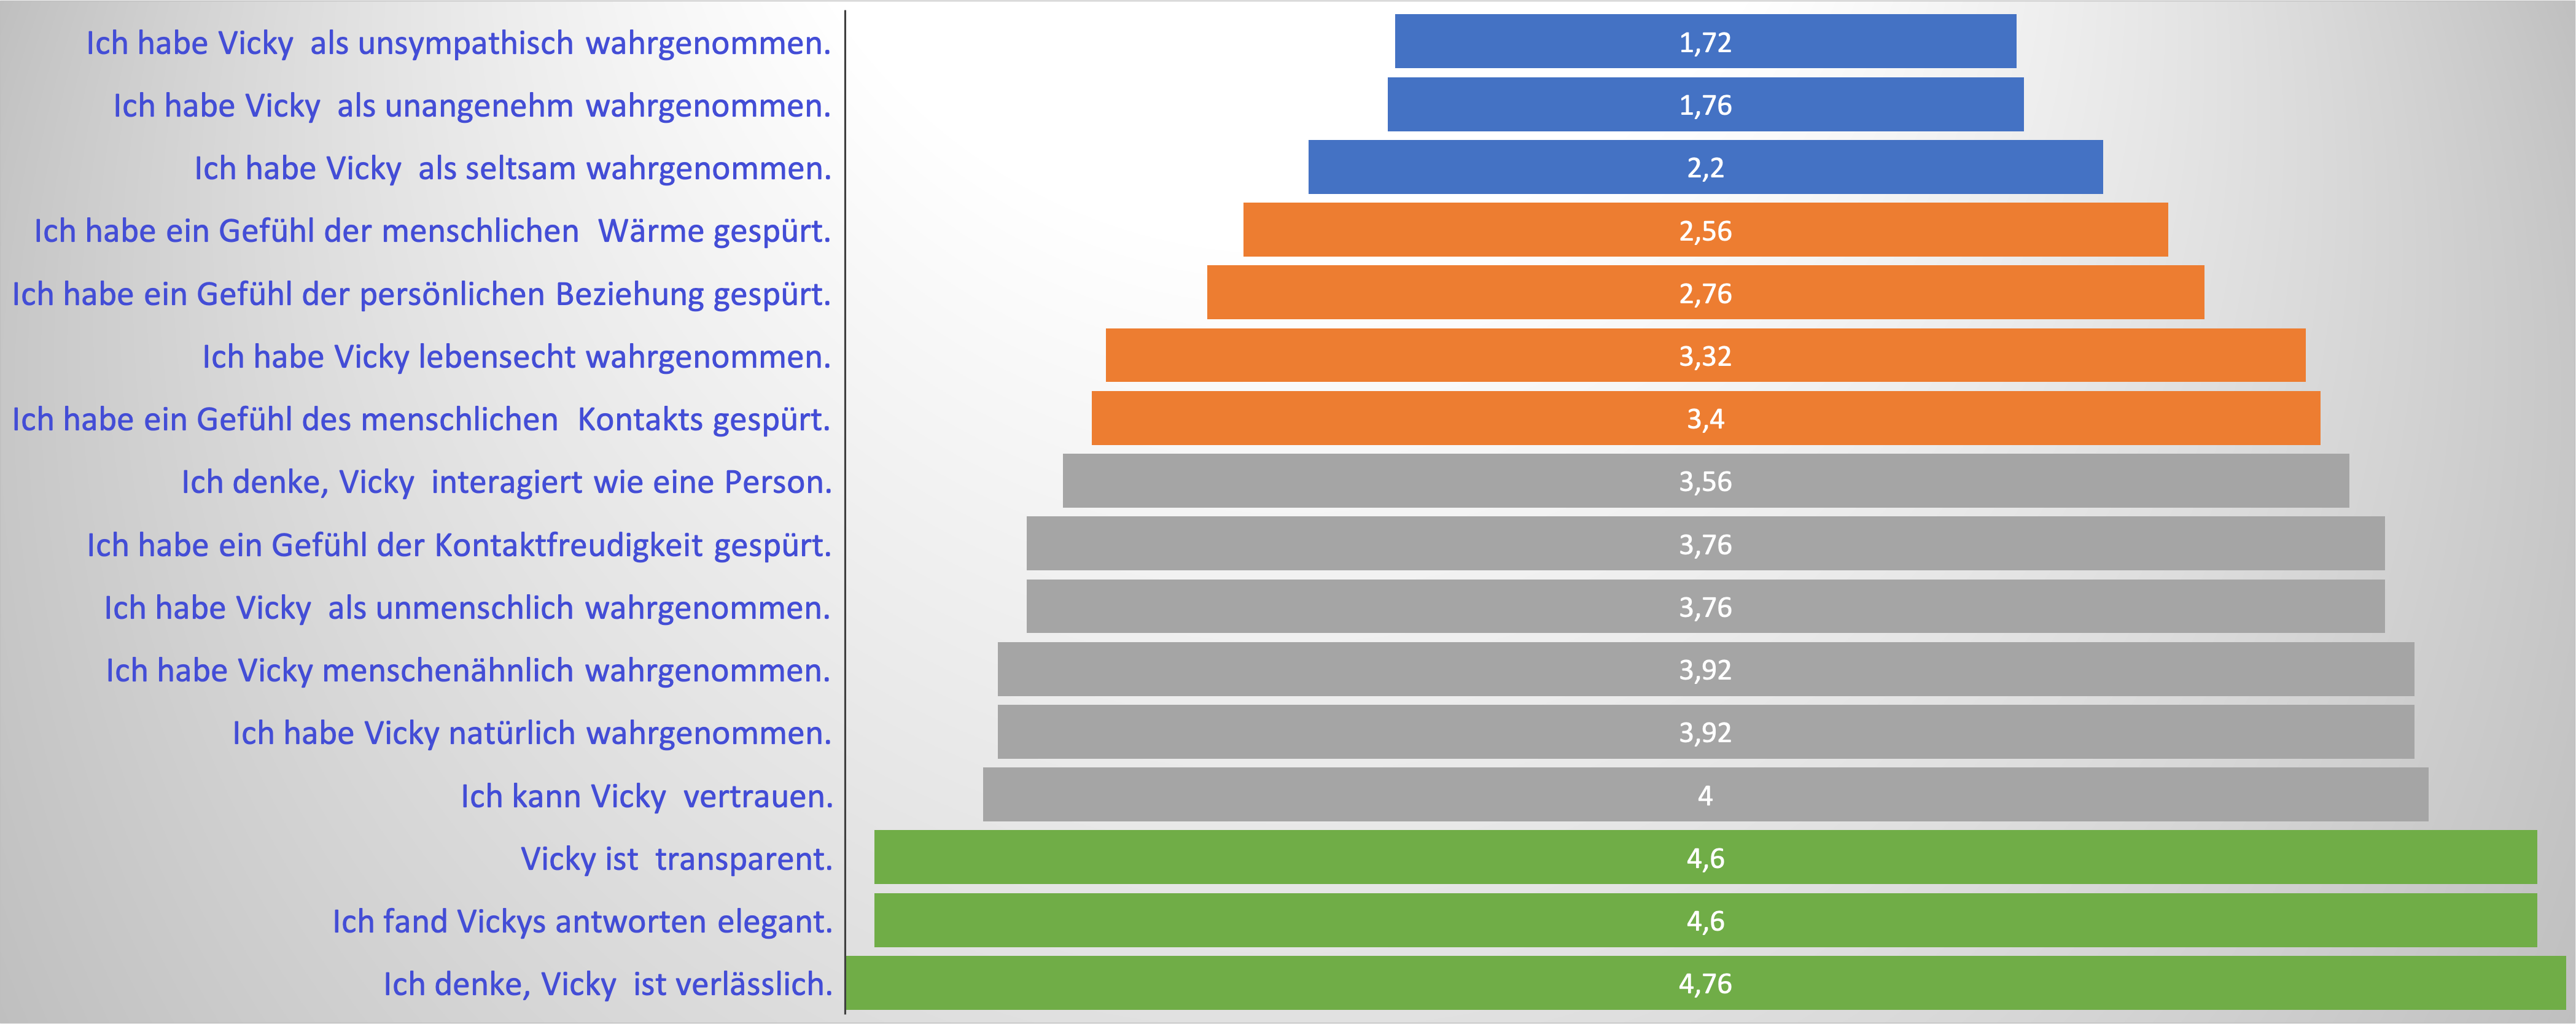
\includegraphics[width=1\linewidth]{images/Auswertung/Wahrnehmung_Vicky.png}
   \caption[Auswertung: Wahrnehmung Vicky] {Auswertung: Wahrnehmung Vicky (eigene Darstellung)}
  \label{fig:Wahrnehmung_Vicky}
  \end{figure} 

Auffallend ist, dass Vicky nicht als unsympathisch, unangenehm und seltsam (in Abb.: blau markiert) wahrgenommen wurde (1,72 $\geq$ MW $\leq$ 2,2).
Die eben genannten Items haben insgesamt einen MW von 1,89 (SD = 1,23), somit scheint Vicky nicht negativ und unheimlich empfunden worden zu sein.
Allerdings konnte Vicky den Befragten keine menschliche Wärme, kein Gefühl einer persönlichen Beziehung, kein Anzeichen von lebensecht und kein 
Gefühl eines menschlichen Kontakts (in Abb.: orange markiert) geben (2,56 $\geq$ MW $\leq$ 3,4).
Insgesamt beträgt der MW 3,01 (SD = 1,30) der eben genannten Items und kennzeichnet damit ein im Durchschnitt eher ablehnendes Urteil.
Somit bedarf es hier weiterer Verbesserungen, um einen höheren Grad einer Mensch-zu-Chatbot Beziehung zu erreichen.
Die Entwicklung bestimmter Charaktereigenschaften, wie z.B. Empathie in einem CA, kann
die Wahrscheinlichkeit erhöhen, dass der Nutzer eine Beziehung zu dem CA aufbaut und ein
positives Nutzererlebnis empfindet. \parencite[289 ff.]{Bickmore.2010} \parencite[7 ff.]{Fitzpatrick.2017}
Die Probanden fällten ein besseres Urteil über die folgenden Items: Vicky interagiert wie eine Person, Kontaktfreudigkeit, Menschlichkeit, Menschenähnlichkeit,
Natürlichkeit und Vertrauen (in Abb.: grau markiert) (3,56 $\geq$ MW $\leq$ 4).
Insgesamt zeigen diese Items einen MW von 3,82 (SD = 1,45), wodurch keine ablehnende oder zustimmende Tendenz erkennbar ist 
und somit sich in ein neutrales Stimmungsbild zeigt.
Aus der Korrelationsanalyse ergab sich ein positiver Zusammenhang zwischen der lebensechten und menschenähnlichen Wahrnehmung von Vicky ($\rho$ = 0,963, vgl. Tabelle \ref{tab:/Korrelationsanalyse}).
Somit könnte für eine höhere Beurteilung der Menschenähnlichkeit eine hohe Bewertung der lebensechten Wahrnehmung von Vicky wichtig sein.
Am besten wurde die Transparenz, die eleganten Antworten und die Verlässlichkeit von Vicky (in Abb.: grün markiert) bewertet (4, 6 $\geq$ MW $\leq$ 4,76).
Der gesamte MW der am besten abgeschnittenen Items beträgt 4,65 (SD = 1,30) und zeigt somit im Mittel ein eher zustimmendes Urteil der Probanden auf.

Die nachfolgende Abbildung stellt eine Häufigkeitsverteilung des klassifizierten Lernstils nach der jeweiligen Interaktion dar.
\begin{figure}[H]
    \centering
    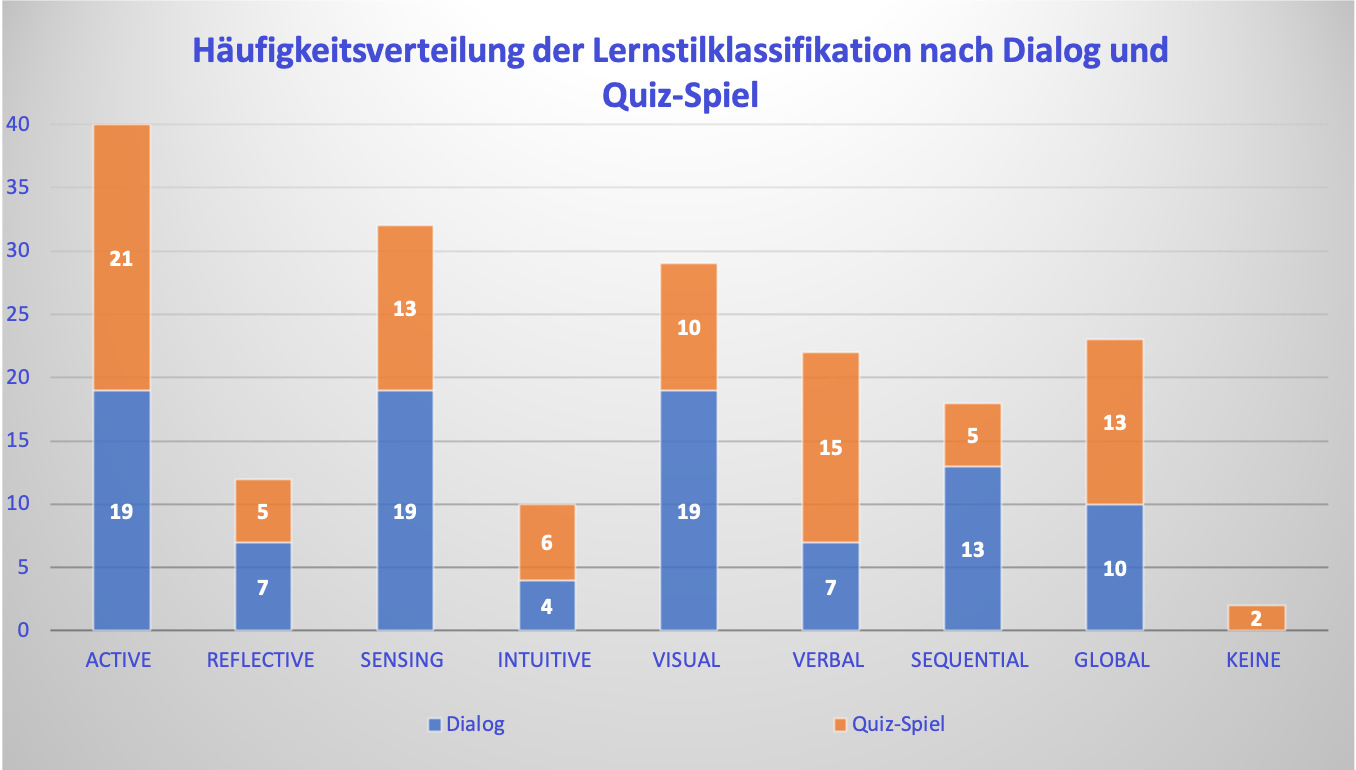
\includegraphics[width=0.65\linewidth]{images/Auswertung/A3.6.png}
   \caption[Auswertung: Häufigkeitsverteilung Lernstilklassifikation] {Auswertung: Häufigkeitsverteilung Lernstilklassifikation (eigene Darstellung)}
  \label{fig:Verteilung_Lernstilklassifikation}
  \end{figure} 

Der sensorische, visuelle, verbale und sequentielle Lernstil zeigt die größten Unterschiede in 
der Anzahl der Klassifizierung auf. 
Dies kann unterschiedliche Gründe aufweisen. Zum einen können die Probanden sehr unterschiedlich im Gespräch und Quiz-Spiel 
interagiert haben. Zum Beispiel könnten die gestellten Fragen im Quiz-Spiel einen anderen Lernstil des Probanden, als im Gespräch identifiziert,
beeinflussen, da zum Beispiel eine Hilfestellung, die dem generellen Lernstils des Probanden nicht entspricht, sich besser eignet um die Frage zu lösen.
 Ein anderer Grund könnte sein, dass nicht alle Quiz-Fragen eigenständig beantwortet wurden, sondern öfter der 
\glqq Solution-Button\grqq{} gedrückt wurde, wobei die Bewertung eines Lernstils entfällt. 
Der aktive, reflektive, intuitive und globale Lernstil wurde sowohl nach dem Gespräch als auch 
nach dem Quiz-Spiel ähnlich häufig klassifiziert.

Etwas weniger als die Hälfte empfand beide Interaktionen (Dialog und Quiz-Spiel) gleich unterhaltsam. 
Knapp ein Drittel der Teilnehmer tendierte zum Dialog. Das Quiz-Spiel gewann die restlichen Probanden (siehe Abbildung \ref{fig:Interaktion_Spaßfaktor}).
\begin{figure}[H]
    \centering
    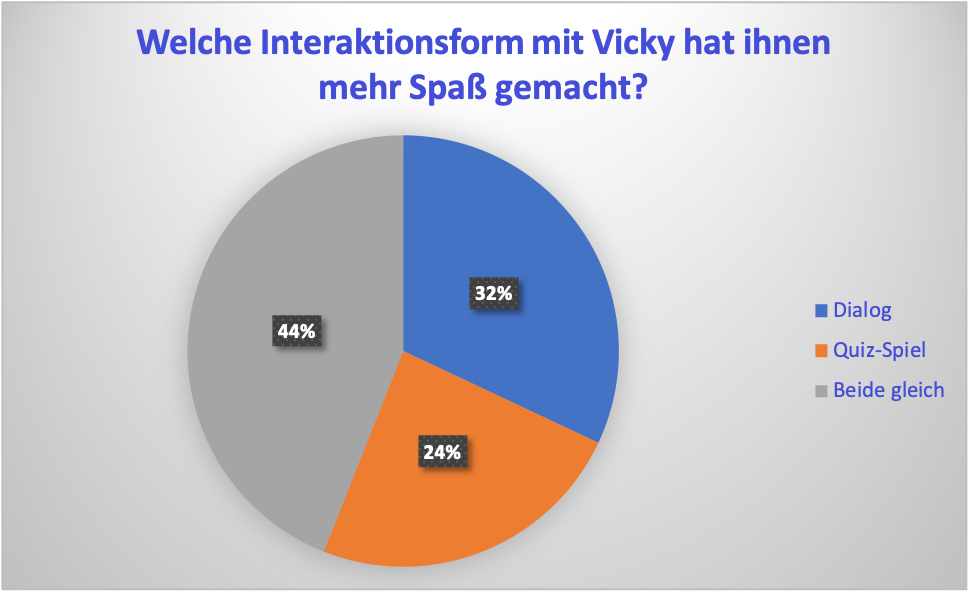
\includegraphics[width=0.6\linewidth]{images/Auswertung/A3.5.png}
   \caption[Auswertung: Spaßfaktor der Interaktionen] {Auswertung: Spaßfaktor der Interaktionen (eigene Darstellung)}
  \label{fig:Interaktion_Spaßfaktor}
  \end{figure} 


Die Tabelle \ref{tab:/Klassifikation_des_Lernstils} zeigt die durchschnittliche Tendenz, inwiefern sich die Beteiligten von Vicky nach der jeweiligen 
Interaktion (Dialog oder Quiz-Spiel) richtig eingeschätzt fühlten.
\begingroup
\footnotesize 
\begin{longtable}{|m{5cm}|m{5cm}|}
    \hline
    \rowcolor[HTML]{EFEFEF} 
    \centering \textbf{Interaktion} &\centering  \arraybackslash \textbf{MW (SD)}\\    \hline \hline
    \centering  Dialog  &  \centering  \arraybackslash  5,24 (1,20)                       \\ \hline
    \centering Quiz-Spiel  &  \centering  \arraybackslash  4,74 (1,39)    \\ \hline
    \caption[Auswertung: Klassifikation des Lernstils MW (SD)]{Auswertung: Klassifikation des Lernstils MW (SD) (eigene Darstellung)} 
    \label{tab:/Klassifikation_des_Lernstils}
\end{longtable}
\endgroup

Im Durchschnitt stimmten die Befragten dem von Vicky klassifizierten Lernstil sowohl nach dem Dialog
als auch nach dem Quiz-Spiel eher zu (4,74 $\geq$ MW $\leq$ 5,24). 
Die Zustimmung zur Lernstilklassifikation nach dem Dialog tendierte in größerer Mehrheit als zum Quiz-Spiel. Die Korrelationsanalyse
ergab einen positiven Zusammenhang zwischen dem Charakterzug Verlässlichkeit und der Tendenz, inwiefern sich die 
Probanden nach der jeweiligen Interaktion (Dialog: $\rho$ = 0,930, Quiz-Spiel:
$\rho$ = 0,695, vgl. Tabelle \ref{tab:/Korrelationsanalyse}) richtig eingeschätzt fühlten. Daher könnte eine verlässliche Wahrnehmung 
eine höhere Glaubwürdigkeit erzeugen.
Zusammenfassend fanden 24 (96 \%) von 25 Teilnehmer sich als richtig eingeschätzt und kommentierten, 
dies sei eine \glqq sehr gute und realistische Einschätzung
meines Lernstils\grqq{} sowie \glqq Ich denke mein Lernstil wurde überwiegend gut eingeschätzt und getroffen\grqq{} (vgl. Anhang \ref{tab:/Kommentare_Teilbereich_2}: 17, 18).


Die positiven und negativen Aspekte über Vicky wurden in Kategorien zusammengefasst (vgl. Anhang \ref{tab:/PostiveAspekte} \& \ref{tab:/NegativeAspekte} ).

\textbf{Positive Aspekte:}

\begin{minipage}[t]{0.5\textwidth}
\begin{itemize}
    \item schnell
    \item verständlich
   \item freundlich
 \item hilfsbereit \\
\end{itemize}
\end{minipage}
\hfill
\begin{minipage}[t]{0.5\textwidth}
    \begin{itemize}
   \item Spaß 
   \item motivierend
 \item authentisch\\
\end{itemize}
\end{minipage}

Positiv wurden die Schnelligkeit und die verständlichen sowie kurzen Satz- und Frageformulierungen bei Vicky gewertet (vgl. Anhang \ref{tab:/PostiveAspekte}: 1, 2, 4, 5, 10, 14).
Des Weiteren trugen die hervorgehobenen Markierungen in den Fragen von Vicky und der intuitive Umgang mit Vicky zu einer höheren Verständlichkeit bei (vgl. Anhang \ref{tab:/PostiveAspekte}: 4, 6, 11, 17). 
Ein weiterer positiver Aspekt ist Vickys Hilfsbereitschaft, die sich in der Erklärung zum Lernstil und in den Hilfestellungen beim Quiz-Spiel zeigten (vgl. Anhang \ref{tab:/PostiveAspekte}: 5, 10, 12, 16, 19).
Außerdem wirkte Vicky freundlich und motivierend, was den Spaßfaktor bei der Interaktion steigerte (vgl. Anhang \ref{tab:/PostiveAspekte}: 7, 8, 11, 13, 14, 16, 17, 18, 19, 20).
Zudem wurden die persönliche Ansprache, die menschliche Umgangssprache und die Möglichkeit zum Smalltalk, wodurch Vicky authentisch wirkte, als positiv gesehen (vgl. Anhang \ref{tab:/PostiveAspekte}: 3, 6, 12, 13, 15).

\pagebreak

\textbf{Negative Aspekte:}

\begin{minipage}[t]{0.5\textwidth}
    \begin{itemize}
    \item unflexibel
    \item unmenschlich
    \item keine Verwendung von Videos/ Bildern \\
\end{itemize}
\end{minipage}
\hfill
\begin{minipage}[t]{0.5\textwidth}
\begin{itemize}
   \item Quiz zu schwer/ zu lang
    \item zeitintensiv\\

\end{itemize}
\end{minipage}

Am meisten wurde die Unflexibilität beim Erkennen der Antworten des Probanden kritisiert (vgl. Anhang \ref{tab:/NegativeAspekte}: 1, 3, 4, 8, 9, 10, 11, 14).
Aufgrund weniger Trainingsdaten,
welche durch diese Umfrage zusätzlich gesammelt wurden, konnte Vicky nicht immer jede Antworteingabe verstehen.
Um möglichst viele Utterances zu bekommen, ist es sinnvoll den Bot so früh wie möglich unter die 
Menschen zu bringen. \footnote{\url{https://rasa.com/docs/rasa-x/user-guide/share-assistant/}, aufgerufen am 15.01.2022 }
Des Weiteren wurde die unmenschliche Wahrnehmung von Vicky als negativ empfunden, die sich zusätzlich 
in der geringen Verwendung von Emotionen zeigte (vgl. Anhang  \ref{tab:/NegativeAspekte}: 2, 9, 13).
Bei einigen Hilfestellungen des Quiz-Spiels wurden Links verschickt,
welche anschließend zu der Video- oder Bild-Hilfestellung führten.
An diese Stelle wäre ein 
direktes Einblenden des Videos oder Bildes wünschenswert gewesen (vgl. Anhang  \ref{tab:/NegativeAspekte}: 6, 7).
Ein weiterer Vorschlag war anstatt der textuellen Erklärung zum Lernstil, eine Erklärung zum Lernstil per Video zu geben,
da die Erklärtexte als zu lang empfunden wurden (vgl. Anhang  \ref{tab:/NegativeAspekte}: 6).
Außerdem wurde der Schwierigkeitsgrad und die Länge des Quiz-Spiels sowie die Kommunikation auf Englisch 
als negativ bewertet (vgl. Anhang  \ref{tab:/NegativeAspekte}: 5, 7, 12).

Zu der Frage, ob es noch weitere Wünsche, Ideen oder Anregungen für die Weiterentwicklung
von Vicky gibt, wurden keine weiteren neuen Anregungen genannt.


\textbf{Deskriptive Auswertung der Fragen zur Lernmotivation (Teilbereich 4): }

Die Tabelle \ref{tab:/ARCS} zeigt die durchschnittliche Tendenz, inwiefern ein CA die Lernmotivation des Befragten beeinflusst hat.
\begingroup
\footnotesize 
\begin{longtable}{|m{5cm}|m{5cm}|}
    \hline
    \rowcolor[HTML]{EFEFEF} 
    \centering \textbf{ARCS-Dimension} &\centering  \arraybackslash \textbf{MW (SD)}\\    \hline \hline
    \centering  A  &  \centering  \arraybackslash  4,85 (1,41)                       \\ \hline
    \centering  R  &  \centering  \arraybackslash  4,29 (1,93)                       \\ \hline
    \centering  C  &  \centering  \arraybackslash  4,64 (1,49)                       \\ \hline
    \centering  S &  \centering  \arraybackslash  4,55 (1,35)    \\ \hline
    \caption[Auswertung: ARCS-Modell MW (SD)]{Auswertung: ARCS-Modell MW (SD)(eigene Darstellung)} 
    \label{tab:/ARCS}
\end{longtable}
\endgroup

Die nachfolgende Abbildung zeigt die Bewertung von den Items der einzelnen ARCS-Dimensionen.
\begin{figure}[H]
    \centering
    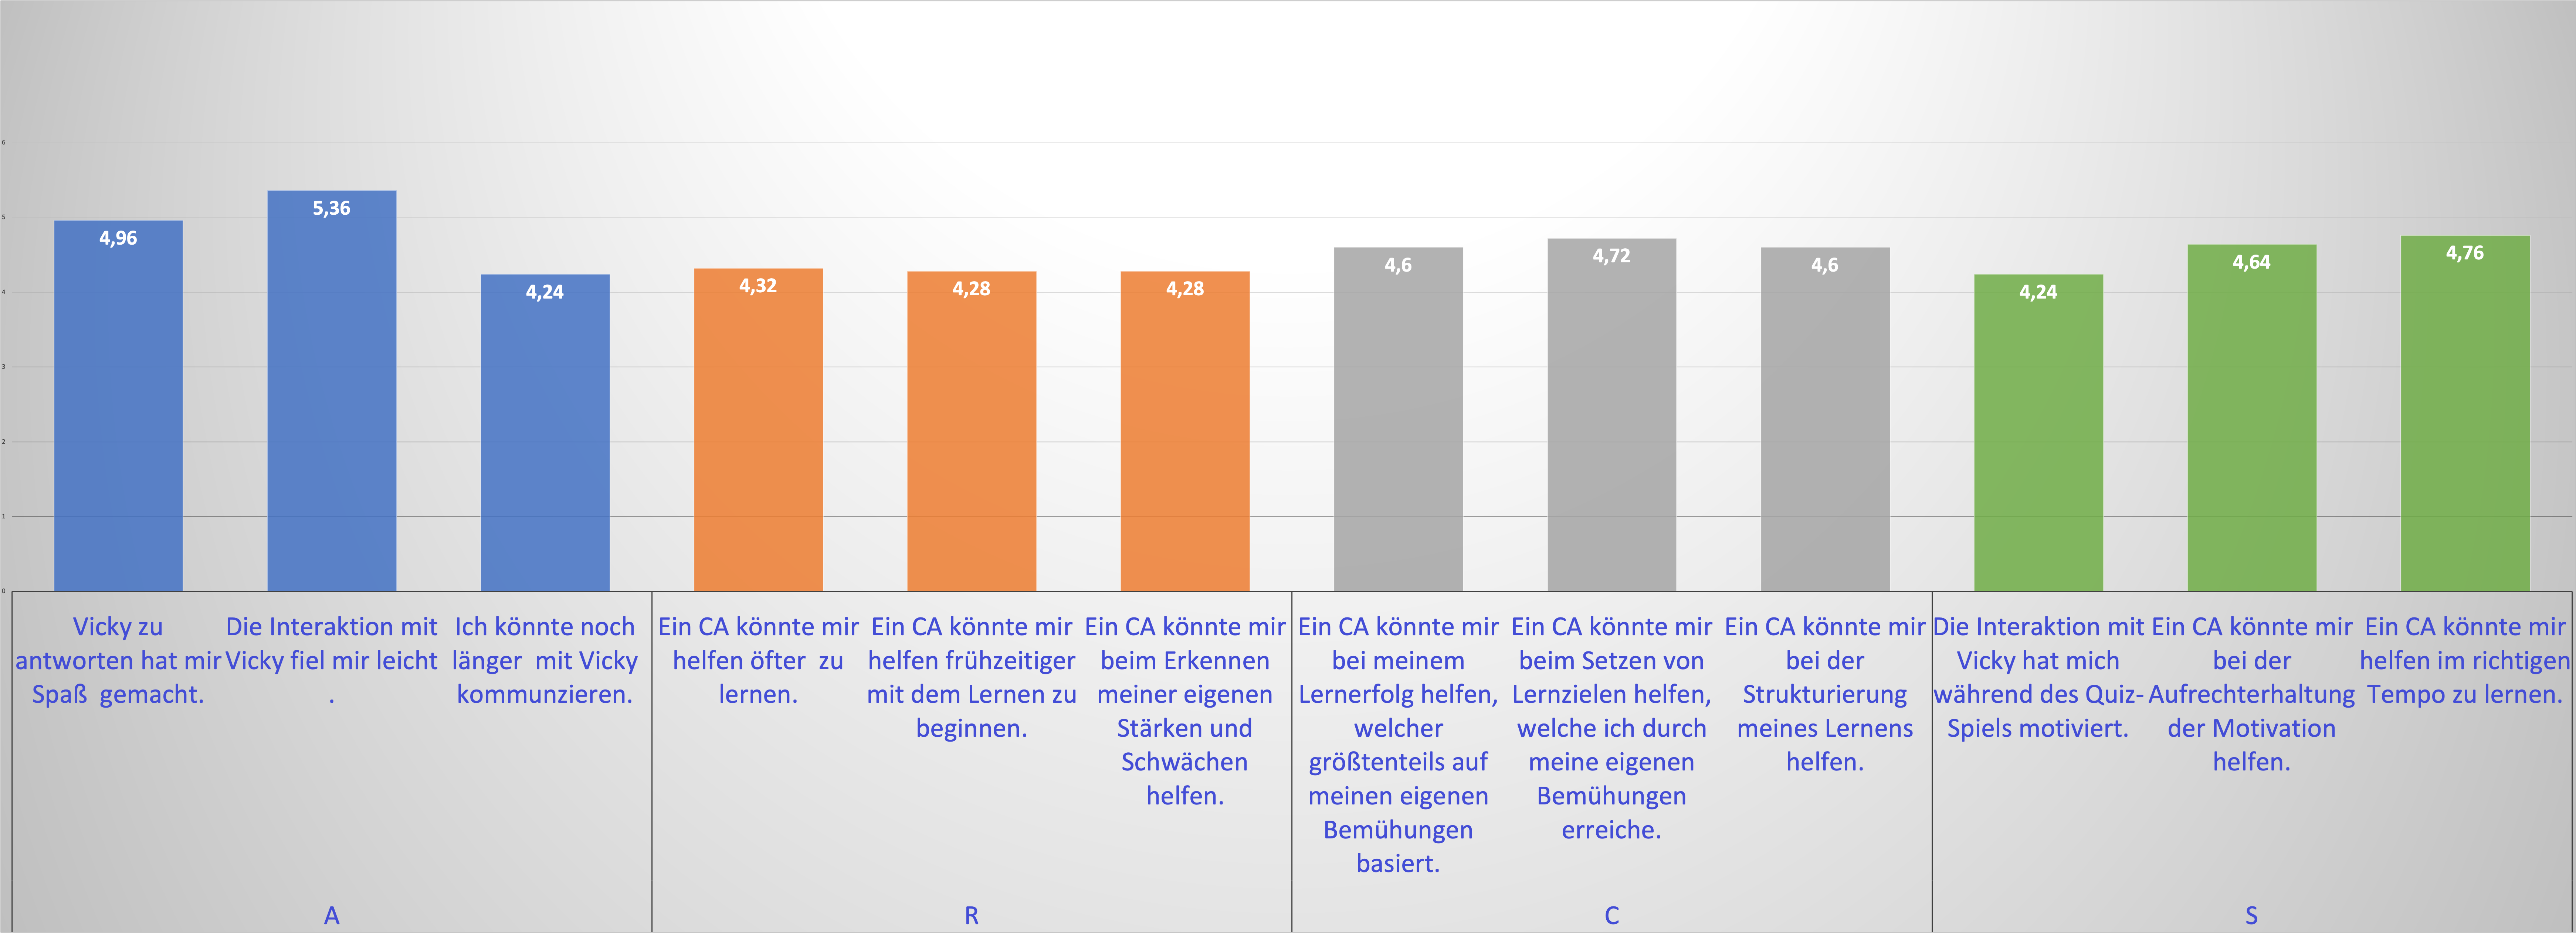
\includegraphics[width=1\linewidth]{images/Auswertung/ARCS.png}
   \caption[Auswertung: ARCS-Dimensionen ] {Auswertung: ARCS-Dimension (eigene Darstellung)}
  \label{fig:ARCS_Dimension}
\end{figure} 

Die folgende Auswertung der Ergebnisse dient der Beantwortung von RQ2 und beziehen sich auf die Abbildung \ref{fig:ARCS_Dimension}
und auf die Tabelle \ref{tab:/ARCS}. 
Außerdem wurden Bezüge zu der im späteren Verlauf beschriebenen Korrelationsanalyse hergestellt (vgl. Tabelle \ref{tab:/Korrelationsanalyse}).\\
Für die Dimension \textbf{Attention (A)} (in Abb.: blau markiert) zeigt sich, dass ein CA die Gunst der Probanden gewinnen kann.
Auffällig ist die positive Bewertung, inwiefern die Interaktion mit Vicky den Teilnehmern leicht fiel und ihnen Spaß gemacht hat.
Dies könnte auf die Korrelation zwischen den eleganten Antworten und dem leichten Umgang mit Vicky zurückgeführt werden, da
diese beiden Variablen positiv korrelieren ($\rho$ = 0,733, vgl. Tabelle \ref{tab:/Korrelationsanalyse}) und die eleganten Antworten von Vicky ebenfalls hoch bewertet wurden.
Ein längeres kommunizieren mit Vicky wurde hingegen nicht direkt gewünscht (siehe Abbildung \ref{fig:ARCS_Dimension}). Dies könnte 
daran liegen, dass die Interaktionen (Gespräch und Quiz-Spiel) mit Vicky in Summe schon eine lange Zeit betrug.
Es besteht eine positive Korrelation ($\rho$ = 0,955) für die Aufrechterhaltung der Kommunikation mit der Kontaktfreudigkeit des CAs (vgl. Tabelle \ref{tab:/Korrelationsanalyse}).
Somit könnte der Charakterzug Kontaktfreudigkeit für eine längere Kommunikation ausschlaggebend sein.
Die Tabelle \ref{tab:/ARCS} zeigt, dass die Dimension Attention im Vergleich zu den anderen Dimensionen am besten abschnitt
und der MW (SD) mit 4,85 (1,41) ein eher zustimmendes Urteil kennzeichnet.

Schlechter stellt sich die Situation für die Dimension \textbf{Relevance (R)} (in Abb.: orange markiert) dar. Sie schneidet im Vergleich zu den 
anderen Dimension am schlechtesten ab (MW (SD) = 4,29 (1,93)). Die Auswertung der einzelnen Items dieser Dimension
zeigt ein neutrales Bewertungsverhalten auf (siehe Abbildung \ref{fig:ARCS_Dimension}). Dies könnte daran liegen, 
dass selbstreguliertes Lernen ein allgemeines großes Motivationsproblem ist (vgl. Kapitel \ref{Problemstellung}),  und die Befragten nicht unbedingt öfter und frühzeitiger 
lernen möchten, sondern eventuell effizienter, sodass weniger Zeit zum Lernen benötigt wird, um den Lernerfolg zu generieren (siehe Abbildung \ref{fig:ARCS_Dimension}).
Für die Identifikation der Stärken und Schwächen könnte ein vertrauensvoller CA von Vorteil sein, da eine 
positive Korrelation ($\rho$ = 0,940) zwischen diesen Variablen besteht (vgl. Tabelle \ref{tab:/Korrelationsanalyse}).

Positiver wurde die Dimension \textbf{Confidence (C)} (in Abb.: grau markiert) bewertet (MW (SD) = 4,64 (1,49)).
Die Teilnehmer zeigten ein Interesse am Lernerfolg, beim Setzen von Zielen sowie an einer Strukturierung des Lernens. 
Diese Aspekte sind Bestandteil des selbstregulierten Lernens und könnten somit 
dieses positiv beeinflussen (vgl. Kapitel \ref{selbstgesteurtesLernen}) und ggf. ein effizienteres 
Lernen ermöglichen.
Aus der Korrelationsanalyse ergab sich ein positiver Zusammenhang zwischen einem verlässlichen CA und der 
Hilfe bei der Strukturierung des Lernens ($\rho$ = 0,941, vgl. Tabelle \ref{tab:/Korrelationsanalyse}). Somit könnte die Verlässlichkeit eine wichtige
charakteristische Eigenschaft darstellen.

Die Tabelle \ref{tab:/ARCS} zeigt für die Dimension \textbf{Statisfaction (S)} (in Abb.: grün markiert)
insgesamt ein eher zustimmendes Ergebnis auf (MW (SD) = 4,55 (1,35)). Am stärksten wurde die Unterstützung des CAs
bezüglich des richtigen Lerntempos bewertet. Ein Grund dafür könnte sein, dass der Lernende durch ein
auf ihn abgestimmtes Lerntempo vor der Überforderung des Lerninhalts bewahrt wird (vgl. Kapitel \ref{Problemstellung}). 
Ebenfalls positiv wurde die Aufrechterhaltung der Motivation beurteilt.
Die Korrelationsanalyse ergab, je menschlicher ein CA ist, desto länger kann die Motivation aufrecht gehalten werden ($\rho$ = 0,977, vgl. Tabelle \ref{tab:/Korrelationsanalyse}).
Somit könnte der menschenähnliche Charakterzug von Bedeutung sein.
Am schlechtesten wurde die motivationale Unterstützung von Vicky während des Quiz-Spiels bewertet.
Möglicherweise wäre es günstiger, nicht nur sachliche Hinweise als Hilfestellungen zu geben, sondern auch motivierende Worte.

Zusammenfassend ist festzuhalten, dass bis auf die Relevance-Dimension, die neutral bewertet wurde,
den drei weiteren Dimensionen positiv zugestimmt wurde. Am höchsten wurde die Attention-Dimension bewertet. Grundsätzlich besteht eine
motivierende Wirkung des CAs auf die Lernmotivation. Allerdings muss hervorgehobenen werden, dass es sich aufgrund 
der geringen Stichprobe nur um erste Tendenzen 
handelt.
\pagebreak

%Teil2 
Die nächste Darstellung zeigt, inwiefern ein CA den \textbf{situativen Faktor} des Rahmenmodells von Rheinberg u.a. (2000) beeinflusst.
\begin{figure}[H]
    \centering
    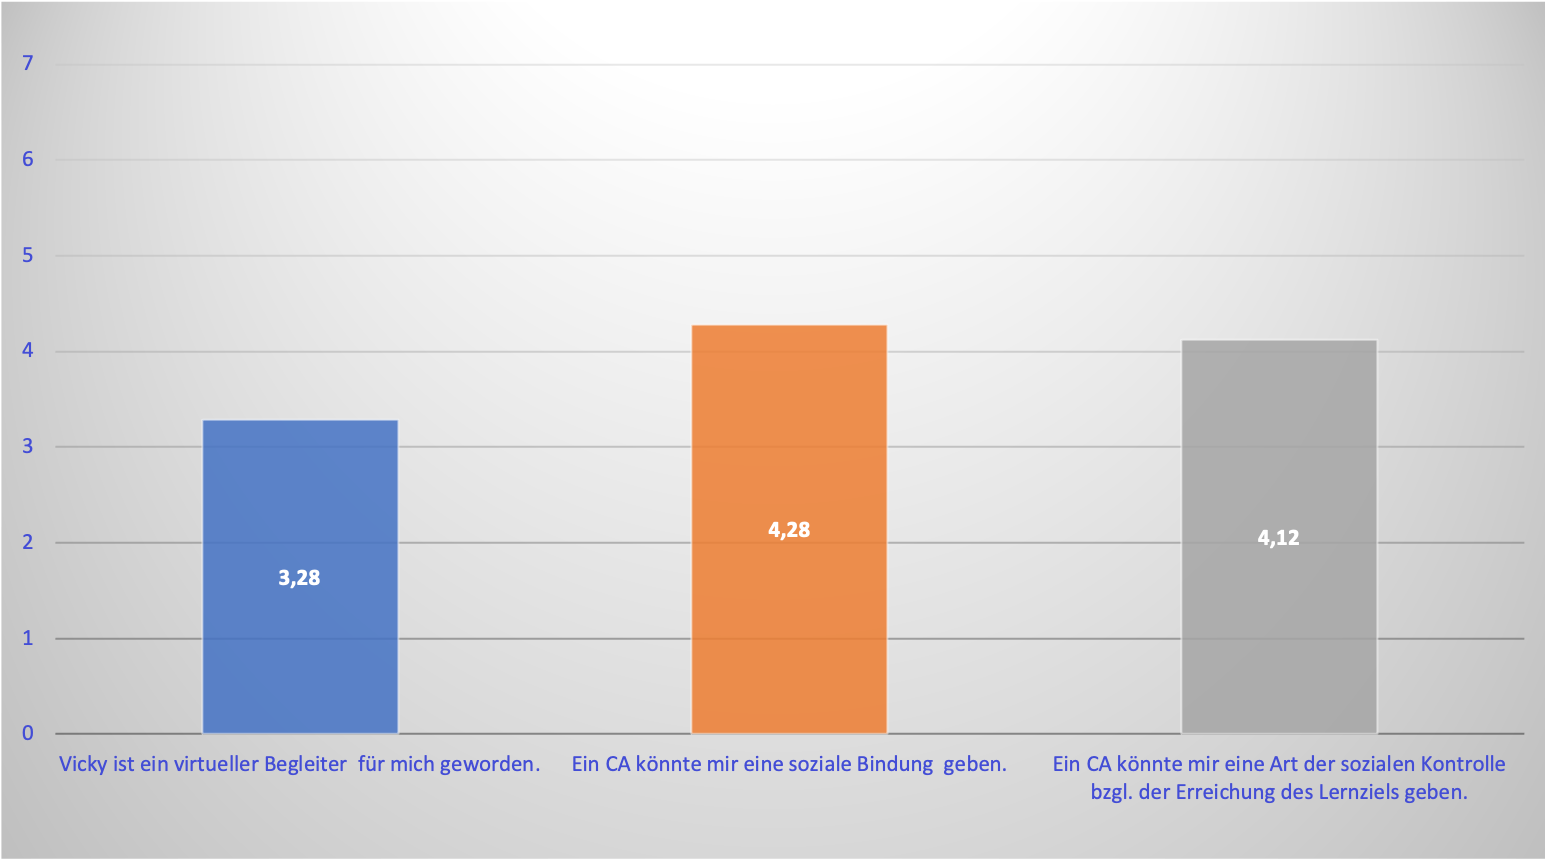
\includegraphics[width=0.9\linewidth]{images/Auswertung/RM.png}
   \caption[Auswertung: situativer Faktor ] {Auswertung: situativer Faktor (eigene Darstellung)}
  \label{fig:RM}
\end{figure} 
Vicky konnte kein virtueller Begleiter des Probanden werden (in Abb.: blau markiert). Dies könnte daran liegen, dass es mehr Zeit und ein häufigeres 
Interagieren zwischen CA und Proband benötigt, um von einem virtuellen Begleiter sprechen zu können.
Positiver wurden die Möglichkeiten, bewertet, dass ein CA eine soziale Bindung und eine Art soziale Kontrolle geben könnte (in Abb.: orange und grau markiert).
Dies zeigt, dass ein Interesse an einem sozialen Austausch besteht. 

Zum Abschluss folgen nun die Auswertung der letzten beiden offenen Fragen.
Zuerst wurden die Teilnehmer befragt, inwiefern sie das Gespräch mit Vicky als motivierend (in Abb.: grün markiert) oder unmotivierend (in Abb.: rot markiert) wahrgenommen hatten.
Dazu wurden aus den 14 Antworten der Teilnehmer Kategorien gebildet. 
Die Antworten der Probanden wurden in eine spielerische Komponente (m), spielerische Komponente (um) und 
Dialog (m) unterteilt (vgl. Anhang  \ref{tab:/VIMUM}). \footnote{m: motivierend, um: unmotivierend}
Die nachfolgende Abbildung zeigt die Häufigkeitsverteilung der Antworten.
\begin{figure}[H]
    \centering
    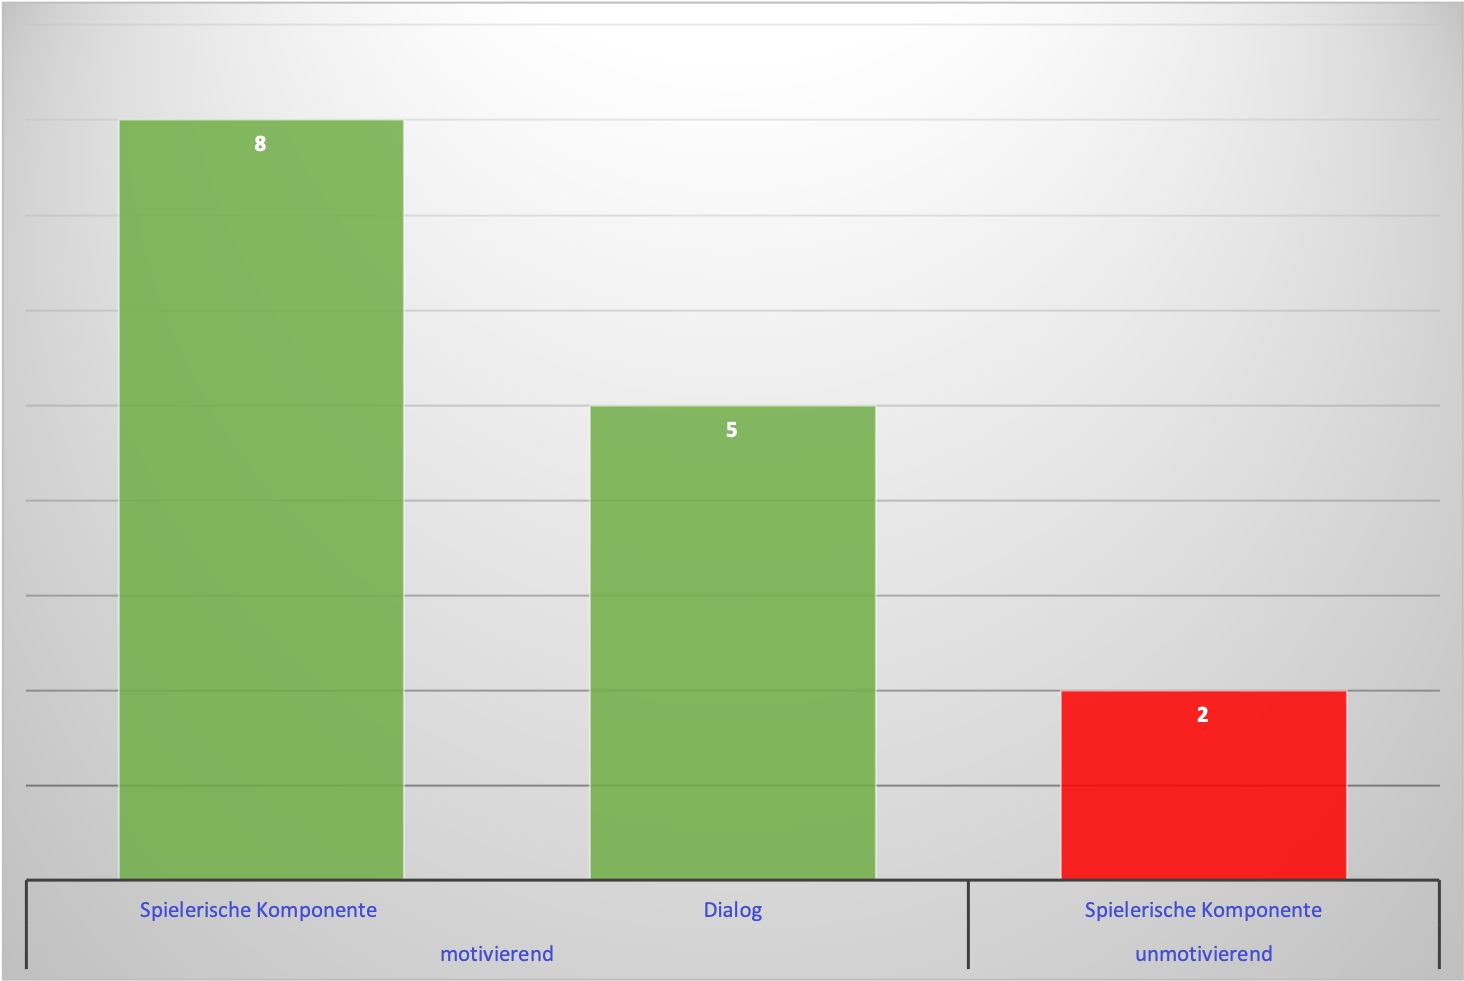
\includegraphics[width=0.8\linewidth]{images/Auswertung/OFLM.png}
   \caption[Auswertung: Häufigkeitsverteilung motivierend/ unmotivierend] {Auswertung: Häufigkeitsverteilung motivierend/ unmotivierend (eigene Darstellung)}
  \label{fig:HMUM}
\end{figure} 
Es ist deutlich zu erkennen, dass der Großteil der Teilnehmer die Interaktion mit Vicky als motivierend empfand.
Das Quiz-Spiel als spielerische Komponente wurde am häufigsten als motivierender Faktor genannt (vgl. Anhang  \ref{tab:/VIMUM}: 1, 2, 4, 6, 7, 9, 13, 14).
Die Hilfestellung und das positive Feedback von Vicky beim Quiz-Spiel waren ausschlaggebende Gründe. Die Unterstützung von Vicky
hat den Probanden beim Herausfinden der richtigen Lösung weit genug in die richtige Richtung gewiesen, um eigenständig antworten zu können (vgl. Anhang  \ref{tab:/VIMUM}: 6, 7, 9, 14).
Außerdem wurde das Quiz-Spiel als nicht so langweilig empfunden wie normales Lernen,
sodass richtig zu antworten aus eigenem Antrieb (intrinsische Motivation) als motivierend empfunden wurde (vgl. Anhang  \ref{tab:/VIMUM}: 2, 4).
Die motivierende Wirkung des Quiz-Spiels ist auf die positiven Auswirkungen von Gamification zurückzuführen (vgl. Kapitel \ref{Forschungsmotivation}).
Dennoch wurde die spielerische Komponente auch als unmotivierend wahrgenommen, da die Quiz-Fragen zu schwer waren, 
oder die Antwort \glqq wrong answer\grqq{} als unmotivierend empfunden wurde (vgl. Anhang  \ref{tab:/VIMUM}: 8, 10).
Der Dialog wurde als weiterer motivierender Aspekt genannt, da ein direkter Austausch zusätzlich eine hilfreiche
Kontrolle ist, und das Lernen dadurch angenehmer und spannender gestaltet werden kann (vgl. Anhang  \ref{tab:/VIMUM}: 3, 5, 8, 11, 12).

Bei der letzten Frage wurde nach dem Empfinden einer Anwesenheit eines virtuellen Begleiters beim Lernen gefragt, welcher
noch weitere Funktionalitäten haben könnte als Lernstile zu klassifizieren.	Die 18 Antworten der Probanden wurden in 
Kategorien zusammengefasst (vgl. Anhang  \ref{tab:/VB}). Die Abbildung \ref{fig:vb} stellt die Häufigkeitsverteilung der Antworten dar.
\begin{figure}[H]
    \centering
    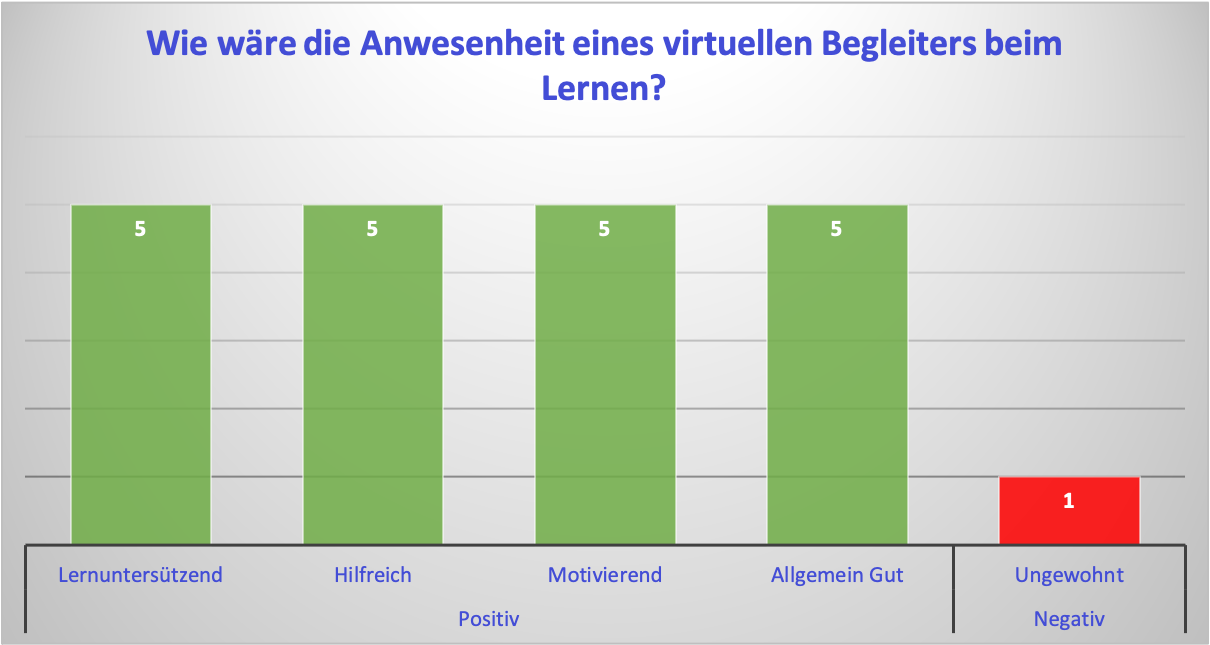
\includegraphics[width=0.8\linewidth]{images/Auswertung/VB.png}
   \caption[Auswertung: Wahrnehmung virtueller Begleiter] {Auswertung: Wahrnehmung virtueller Begleiter (eigene Darstellung)}
  \label{fig:vb}
\end{figure} 
Insgesamt fand der Großteil der Teilnehmer die Anwesenheit eines virtuellen Begleiters positiv,
da sie ihn als lernunterstützend, hilfreich, motivierend und allgemein gut wahrnehmen würden (in Abb.: grün markiert) (vgl. Anhang  \ref{tab:/VB}: 1-15, 17, 18).
Bezogen auf den Aspekt der Lernunterstützung könnte ein virtueller Begleiter helfen, die Lerninhalte
zu strukturieren und aufzuteilen. Außerdem könnte dieser je nach Lernstand passende 
Übungsaufgaben zum Lernthema stellen und Informationen zum Lernthema bereitstellen,
sodass ein besserer Lernerfolg erzielt werden kann (vgl. Anhang  \ref{tab:/VB}: 4, 7, 13).
Des Weiteren wurde vorgeschlagen, dass ein virtueller Begleiter 
sowohl eine Hilfe im Zeitmanagement sein kann, zur
Unterstützung beim Bilden von Lerngruppen mit gleichem Lernstil dienen könnte
als auch eine Form der sozialen Kontrolle sein könnte, sodass es leichter fällt 
stetig zu lernen (vgl. Anhang  \ref{tab:/VB}: 14, 17).
Ein virtueller Begleiter kann hilfreich sein für generelle Fragen des Studierenden,
zu einer besseren Orientierung im Studium, gerade für Studienanfänger, sowie
unterstützend sein beim Erstellen des Lernplans (vgl. Anhang  \ref{tab:/VB}: 8, 18).
Dennoch würde ein Teilnehmer einen virtuellen Begleiter als ungewohnt empfinden (in Abb.: rot markiert) (vgl. Anhang  \ref{tab:/VB}: 16).
Ferner können diese Wünsche und Anregungen für weitere Folgearbeiten anregen.

\pagebreak

\textbf{Korrelationsanalyse}

Im Folgenden wird das Ergebnis einer Korrelationsanalyse aufgeführt. 
Diese Analyse dient dazu, Tendenzen in Bezug auf die Zusammenhänge zwischen den 
in der Tabelle \ref{tab:/Korrelationsanalyse} betrachteten 
Items zu erkennen und neues Wissen über die Wahrnehmung von CAs zu generieren.
Für die Auswertung wird die Spearman-Korrelation verwendet, da die Variablen (Items)  intervallskaliert sind.
Es wird durchgängig ein Signifikanzniveau von $\alpha$ = 0,01 verwendet.

\begingroup
\footnotesize 
\begin{longtable}{|m{5.5cm}|m{5.5cm}|m{3cm}|}
    \hline
    \rowcolor[HTML]{EFEFEF} 
    \centering \textbf{Item 1} &\centering \textbf{Item 2} & \centering \arraybackslash \textbf{$\rho$}\\    \hline \hline
    Erfahrung im Umgang mit Chatbots & Ich habe Vicky als unmenschlich wahrgenommen.  & \centering \arraybackslash 0,974    \\ \hline
    Ich habe Vicky als lebensecht wahrgenommen. & Ich habe Vicky als menschenähnlich wahrgenommen.  & \centering \arraybackslash 0,963                      \\ \hline
    Ich denke, Vicky ist verlässlich. & Lernstileinschätzung Dialog  & \centering \arraybackslash 0,930                      \\ \hline
    Ich denke, Vicky ist verlässlich.&  Lernstileinschätzung Quiz-Spiel & \centering \arraybackslash 0,695                      \\ \hline
    Ich habe Vicky als seltsam wahrgenommen. & Ich habe Vicky als unmenschlich wahrgenommen.  & \centering \arraybackslash 0,891                      \\ \hline
    Ich fand Vickys Antworten elegant. & Die Interaktion viel mir mit Vicky leicht.  & \centering \arraybackslash 0,733                      \\ \hline
    Ich hab eine Gefühl der Kontaktfreudigkeit gespürt. & Ich könnte noch länger mit Vicky kommunizieren.  & \centering \arraybackslash  0,955                      \\ \hline
    Ich kann Vicky vertrauen. & Ein CA könnte mir beim Erkennen meiner eigenen Stärken und Schwächen helfen. & \centering \arraybackslash 0,940                      \\ \hline
    Ich denke Vicky ist verlässlich.  & Ein CA könnte mir bei der Strukturierung meines Lernens helfen.  & \centering \arraybackslash 0,941                      \\ \hline
    Ich habe Vicky menschenähnlich wahrgenommen. & Ein CA könnte mir bei der Aufrechterhaltung der Motivation helfen.  & \centering \arraybackslash 0,977                      \\ \hline
    \caption[Korrelationsanalyse] {Korrelationsanalyse (eigene Darstellung)}
    \label{tab:/Korrelationsanalyse}
\end{longtable}
\endgroup

Für jedes aufgeführte Itempaar der Tabelle \ref{tab:/Korrelationsanalyse} besteht ein (positiver) signifikanter Zusammenhang.
Nach Cohen (1988) ist der Effekt als stark einzuordnen, da alle Korrelationskoeffizienten ($\rho$) über 0,5 liegen. \parencite[80]{Cohen.1988}
Demnach kann davon ausgegangen werden, dass die Erfahrung im Umgang mit Chatbots einen Einfluss darauf hatte, wie gut oder schlecht 
Vicky als unmenschlich wahrgenommen wurde.
Weitere Aspekte \footnote{Anzumerken ist, dass bei einer starken Korrelation nicht gesagt werden kann, welche das abhängige und 
welche das unabhängige Item ist. Dadurch kann nicht bestimmt werden, welches Item den Einfluss ausübt. Aus Gründen der besseren Lesbarkeit wird im 
folgenden Item 1 als abhängiges und Item 2 als unabhängiges Item angesehen. Vgl. \url{https://statistikguru.de/spss/spearman-korrelation/spearman-einfuehrung.html}, aufgerufen am 15.01.2022} 
sind, dass je lebensechter Vicky wahrgenommen wurde, desto menschenähnlicher wurde Vicky bewertet,
je verlässlicher Vicky eingeschätzt wurde, desto stärker haben sich die Probanden nach dem Dialog und Quiz-Spiel bei ihrer Lernstilidentifikation richtig eingestuft gefühlt, 
je seltsamer Vicky wahrgenommen wurde, desto unmenschlicher wurde Vicky eingestuft, je eleganter 
Vickys Antworten empfunden wurden, desto leichter viel dem Probanden die Interaktion mit Vicky, je stärker ein Gefühl 
der Kontaktfreudigkeit gespürt wurde, desto länger konnte der Befragte mit Vicky kommunizieren, 
je stärker Vicky vertraut werden konnte, desto besser könnte ein CA bei der Strukturierung des Lernens helfen und 
je menschenähnlicher Vicky wahrgenommen wurde, desto länger konnte die Motivation aufrechterhalten werden.
Diese Korrelationen können für die Weiterentwicklung berücksichtigt werden, um bestimmte Wirkungen besser oder schlechter zu generieren.

\textbf{Kapitelzusammenfassung} 
\begin{itemize}
    \item Der Aufbau und die Itemauswahl des Studiendesigns wurden ausführlich in Kapitel \ref{Kapitel5.1} beschrieben. Die Auswertung der Umfrage (Kapitel \ref{Kapitel5.2}) ergab wichtige Erkenntnisse und Tendenzen zur Beantwortung von RQ1 und RQ2.
    \item Vicky wurde im Allgemeinen nicht als negativ und unheimlich empfunden. Dennoch konnte Vicky noch nicht in den Aspekten Menschenähnlichkeit und Aufbau einer persönlichen Beziehung 
überzeugen. Am positivsten wurde die Verlässlichkeit von Vicky bewertet. Dennoch sind Weiterentwicklungen von Vicky für eine menschenähnlichere Wahrnehmung notwendig.
    \item Die Probanden gaben eine positive Tendenz, dazu ab, dass die individuelle Lernstilklassifikation sowohl nach dem Dialog als auch nach dem Quiz-Spiel auf sie zuträfe, wobei der Dialog eine größere Mehrheit an Zustimmung bekam. Insgesamt fühlten sich 24 von 25 Teilnehmern richtig eingeschätzt.
    \item Positiv wurden die Schnelligkeit und die verständlichen sowie kurzen Satz- und Frageformulierungen bei Vicky gewertet. Des Weiteren wirkte Vicky freundlich, hilfsbereit, motivierend und authentisch.
    \item Am meisten wurde die Unflexibilität beim Erkennen der Antworten des Probanden kritisiert. Zudem wurde die unmenschliche Wahrnehmung von Vicky als negativ empfunden.
    Bei einigen Hilfestellungen des Quiz-Spiels wäre ein direktes Einblenden des Videos oder Bildes wünschenswert gewesen, anstatt das Verschicken eines Links.
    Des Weiteren wurde anstatt der textuellen Erklärtexte zum Lernstil eine Erklärung im Videoformat gewünscht.
    Außerdem wurde der Schwierigkeitsgrad und die Länge des Quiz-Spiels sowie die Kommunikation auf Englisch als negativ bewertet.
    \item Die Lernmotivation wurde mithilfe des ARCS-Modells gemessen. Bis auf die Relevance-Dimension, welche eine neutrale Zustimmung bekam, konnte für die weiteren drei Dimensionen eine positive Tendenz gemessen werden.
    \item Vicky wurde nicht als virtueller Begleiter akzeptiert, dennoch besteht Interesse auf weiteren sozialen Austausch sowie Vicky als motivierend empfunden wurde.
    \item Die Anwesenheit eines virtuellen Begleiters wurde als positiv empfunden, da er das Lernen unterstützen kann und die Probanden ihn als hilfreich und motivierend wahrnehmen würden. Zudem wurden interessante Vorschläge zu weiteren Einsatzgebieten des virtuellen Begleiters gemacht.
    \item Mithilfe einer Korrelationsanalyse wurden Annahmen für Begründungen von bestimmten Wirkungszusammenhängen getroffen.
\end{itemize}

